\cleardoubleoddpage
\chapter{Results}
\label{app:results}

In this chapter, we analyze the performance of both the Supervised BC classifier models, developed for use as regularization terms, and the offline DQN+BC agents that were trained using these BC models. The discussion focuses on how the choice of dataset affects model performance, the effects of state normalization, and overall behaviour in the online environment. Emphasis is placed on analyzing observed differences due to dataset composition, state normalization, and training methodology, particularly in the context of using pretrained BC models as regularization components in DQN+BC.

The performance of the online environment was evaluated using the accumulated rewards obtained from 1000 episodes with unique random seeds. The mean and SD of these accumulated rewards for each model and agent configuration are reported in Table \ref{tab:bc_live_env_mean_std}. In addition, KDE distributions of accumulated rewards are presented in Figure \ref{fig:BC_live_env_evaluation} for the supervised BC classifiers and in Figure \ref{fig:DQN_BC_live_env_evaluation} for the DQN+BC configurations. Due to the high variance and multimodal structure of the accumulated reward distributions, observed both during data exploration and in the results presented here, the mean alone is not a sufficient metric for performance evaluation. Consequently, a careful examination of the full KDE accumulated reward distributions is required to obtain a more reliable and informative evaluation of each agent`s behaviour.

\section{Performance of Supervised BC Models}
Before analyzing the performance of the offline DQN+BC agents, we first investigate the supervised BC classifiers trained separately and specifically for use in the proposed regularization framework. These BC models can be examined in two complementary directions: their ability to imitate the original online DQN agents and their performance in the online environment. Since they were trained for use as regularization components rather than as standalone agents, greater emphasis is placed on their imitation performance.

Imitation performance was evaluated using standard classification metrics, including accuracy, balanced accuracy, weighted precision, recall, and F1-score, with balanced accuracy serving as the main evaluation metric. All imitation metrics were computed on a held-out test dataset that was not used during training nor hyperparameter tuning. These metrics for each normalization and dataset variation of the imitation BC models can be found in Table \ref{tab:bc_evaluation_metrics}.

Although supervised BC models were also evaluated in the online environment, this evaluation was mainly used for qualitative comparison rather than as an optimization objective, given that these models were designed to function as regularization components rather than as standalone agents.




\begin{table}[!ht]
\centering
\caption{Evaluation metrics of supervised BC models on the test sets for RB and FP datasets across different state normalization techniques.}
\label{tab:bc_evaluation_metrics}

\renewcommand{\arraystretch}{1.2}  % increase row height

\begin{tabular}{p{1.5cm} c c p{1.75cm} p{1.75cm} p{1.75cm} p{1.75cm}}
\hline
\textbf{Norm.} 
& \textbf{Dataset} 
& \textbf{Accuracy} 
& \textbf{Balanced Accuracy}
& \textbf{Precision (Weighted)} 
& \textbf{Recall (Weighted)} 
& \textbf{F1-score (Weighted)} \\
\hline
Raw        & RB & 0.567 & 0.562 & 0.652 & 0.567 & 0.591 \\
           & FP & 0.984 & 0.984 & 0.980 & 0.979 & 0.980 \\
\hline
Min-Max    & RB & 0.574 & 0.563 & 0.655 & 0.574 & 0.598  \\
           & FP & 0.980 & 0.984 & 0.981 & 0.980 & 0.980 \\
\hline
Max-Abs    & RB & 0.573 & 0.562 & 0.652 & 0.573 & 0.596 \\
           & FP & 0.976 & 0.983 & 0.978 & 0.976 & 0.977 \\
\hline
Robust     & RB & 0.574 & 0.563 & 0.654 & 0.574 & 0.597  \\
           & FP & 0.969 & 0.979 & 0.972 & 0.969 & 0.969 \\
\hline
Standard   & RB & 0.576 & 0.564 & 0.653 & 0.576 & 0.599 \\
           & FP & 0.976 & 0.980 & 0.977 & 0.976 & 0.976  \\
\hline
\end{tabular}
\end{table}


\begin{table}[!ht]
\centering
\caption{Performance of BC and DQN+BC models across normalization methods in the live environment (mean $\pm$ SD over 1000 uniquely seeded episodes).}
\label{tab:bc_live_env_mean_std}

\begin{tabularx}{\textwidth}{%
  p{2cm}                   % first column: Model Type, left-aligned by default
  >{\centering\arraybackslash}p{1.5cm}  % second column: Dataset, centered
  *{5}{>{\centering\arraybackslash}X}   % remaining columns: flexible width, centered
}
\hline
\textbf{Model Type} 
& \textbf{Dataset} 
& \textbf{Raw} 
& \textbf{Max-Abs} 
& \textbf{Min-Max}
& \textbf{Robust}
& \textbf{Standard} \\
\hline
BC (Supervised) & RB &  $-68.46 \pm 66.00$ & $-70.30 \pm 52.49$ & $-110.36 \pm 102.46$ & $-78.09 \pm 73.00$ &$-101.58 \pm 114.18$ \\
                & FP &  $80.62 \pm 105.57$ & $79.45 \pm 106.91$ & $79.30 \pm 106.19$ & $82.46 \pm 105.22$ & $78.27 \pm 107.35$\\
BC-only ($\tau=1$) & RB & $46.11 \pm 128.83$ & $-183.57 \pm 88.16$ & $-957.51 \pm 1405.13$ &  $-62.46 \pm 140.14$ & $10.09 \pm 192.92$\\
           & FP & $-125.81 \pm 200.00$ & $-307.87 \pm 209.02$ & $-289.63 \pm 78.97$ & $-313.57 \pm 140.14$ & $-160.24 \pm 277.97$  \\
DQN+BC ($\tau$ hyperparam) & RB & $-15.64 \pm 125.33$ & $-102.22 \pm 103.47$ & $-873.93 \pm 206.89$ & $164.82 \pm 246.18$ & $52.50 \pm 66.71$ \\
                           & FP & $-344.52 \pm 198.37$ & $-198.37 \pm 206.89$ & $-354.44 \pm 246.87$ & $-133.28 \pm 107.18$ & $696.79 \pm 40.60$ \\
DQN-only ($\tau=0$) & RB & $158.01 \pm 108.12$ & $-139.89 \pm 197.78$ & $-790.27 \pm 368.32$ & $80.27 \pm 124.39$ & $111.88 \pm 81.88$ \\
           & FP & $-472.50 \pm 120.42$ & $-100.30 \pm 76.56$ & $-744.70 \pm 302.64$ & $-437.49 \pm 316.82$ & $-153.15 \pm 78.71$ \\
\hline
\end{tabularx}
\end{table}


\begin{figure}[!b]
\centering
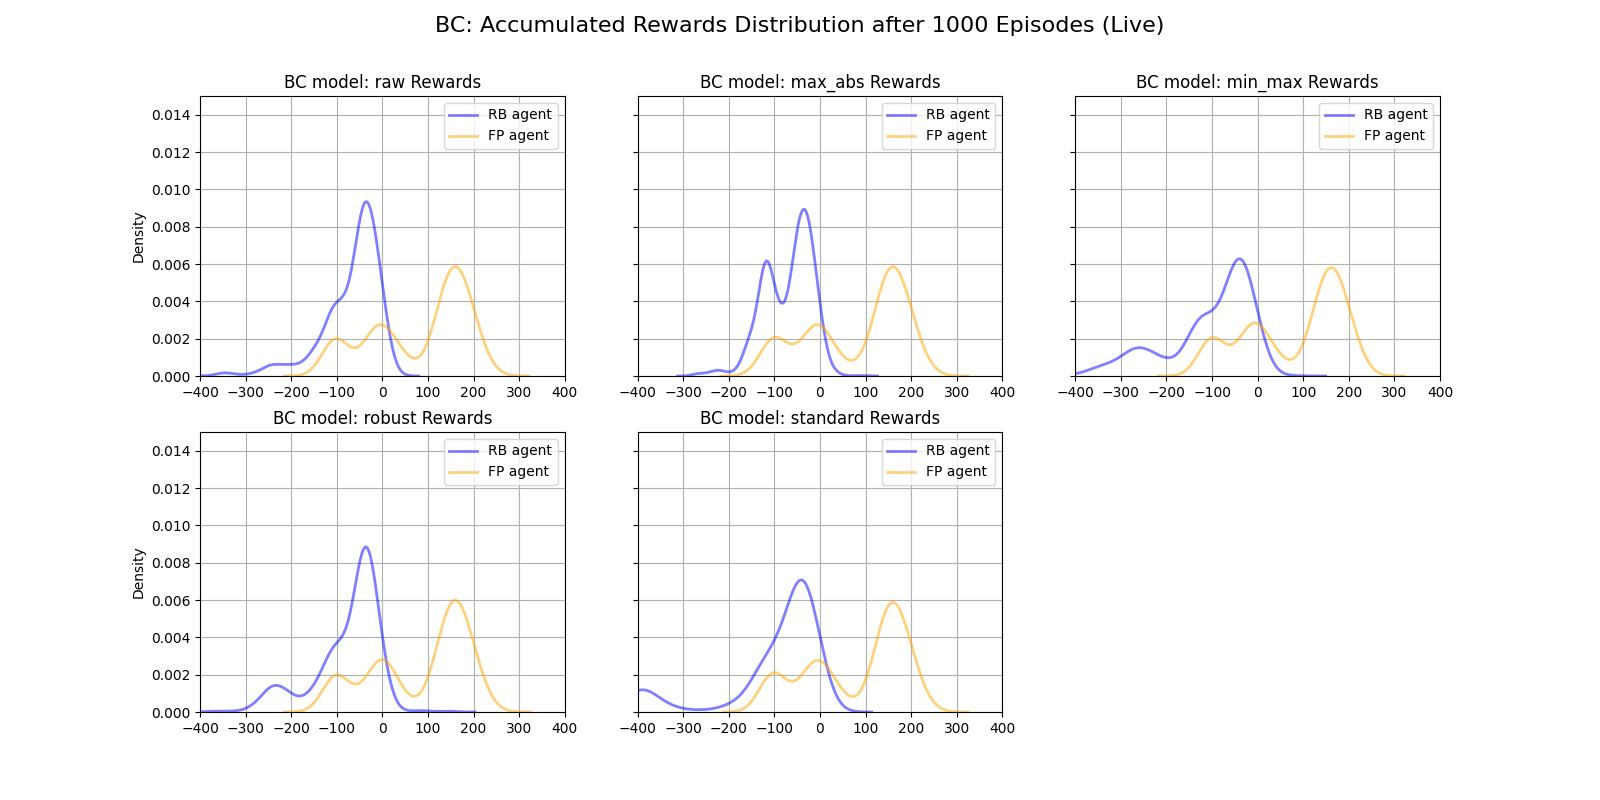
\includegraphics[width=1.1\linewidth]{images/BC_experiments_summary_live_env_1000_ep_eval_rb_fp.jpg}
\caption{
Accumulated reward KDE distributions for Supervised BC models across all normalization and dataset variations, evaluated over 1,000 uniquely seeded live environment episodes. Each model predicts the actions of the original online agent given the current state, framing RL as a supervised learning problem. Distribution plots are restricted to $[-400, 400]$ for clarity.
}
\label{fig:BC_live_env_evaluation}
\end{figure}



\subsection{Impact of Dataset Composition on BC Performance (RB vs FP)}
The composition of the training dataset had a significant effect on the performance of supervised BC models in all evaluation settings. In particular, BC models trained on the FP dataset consistently outperformed those trained on the RB dataset, both in terms of imitation performance on the held-out test subsets and in qualitative evaluation within the online environment, regardless of the applied state normalization technique.

FP BC models achieved balanced accuracy scores of at least $98\%$ across all normalization variants, showing a near-perfect imitation of the behaviour of the original online DQN agent. This strong imitation performance was also reflected in the live environment, where FP BC models produced accumulated reward distributions that closely resembled those of the original FP DQN policy. As shown in Figure \ref{fig:BC_live_env_evaluation}, these distributions exhibited peaks around reward values of approximately $-100$, $0$, and a dominant peak near $150$. Although FP BC models occasionally approached the environment’s reward threshold for a successful episode of $200$, they did not consistently achieve it. This behaviour was expected given their purely supervised training objective and the fact that the original FP DQN agent itself did not reliably surpass the $200$ accumulated reward per episode threshold.

In contrast, BC models trained on the RB dataset performed poorly in both imitation and live environment evaluations. Across all normalization settings, RB BC models achieved balanced accuracy values in a narrow range between $56.2\%$ and $56.4\%$. Their accumulated reward distributions in the live environment differed substantially from those of the original DQN agent and exhibited limited structure, indicating unstable and ineffective learned policies.

This performance gap can be attributed to key differences in dataset composition. The RB dataset consists of state-action pairs generated by multiple sub-optimal policies, which leads to high variability in behaviour and inconsistent action choices for similar states. As a result, supervised learning struggled to extract a single consistent policy from the RB data. This limitation continued even when model capacity was increased - larger RB BC models with more neurons and hidden layers did not yield meaningful improvements in imitation accuracy or live environment performance, suggesting that the dataset itself imposes the main performance constraint.

By contrast, the FP dataset was generated by a single near-optimal and consistent policy, allowing supervised BC models to learn a well-defined state-action mapping. To capture this more consistent policy effectively, FP BC models required more complex architectures with a higher number of hidden neurons and layers compared to RB BC models. This increased capacity directly translated into improved imitation performance and more stable behaviour in the live environment.

Overall, these results demonstrated that FP datasets yielded substantially higher-quality BC models than RB datasets. This held not only for imitation performance and direct live environment evaluation, but also for their suitability as regularization components in offline RL, where accurate and consistent behaviour imitation is critical.







\subsection{Effect of State Normalization on BC Performance}

The application of state normalization techniques had limited effect on the performance of the supervised BC models, regardless of whether they were trained on the RB or FP datasets. Across all normalization variants, imitation performance on the held-out test sets remained largely unchanged, with balanced accuracy values varying by at most $0.1\%$ to $0.5\%$ (Table~\ref{tab:bc_evaluation_metrics}). This indicates that state normalization did not meaningfully influence the supervised learning objective, and the BC models were able to learn the underlying state-action mappings reliably even when trained on raw state representations. This effect was likely due to the large size of both training subsets, each containing more than $800,000$ state-action pairs, which appeared sufficient to allow effective policy generalization even in the absence of additional preprocessing techniques.

For BC models trained on the FP dataset, this lack of sensitivity to normalization was also observed in the online environment (Figure~\ref{fig:BC_live_env_evaluation}). Across all normalization methods, the accumulated reward distributions were very similar, with insignificant differences in their shape or central tendency. This behaviour was consistent with the strong imitation performance of the FP BC models and the consistency of the underlying training data. Since these models already generalized reliably to the online environment, applying state normalization did not lead to noticeable performance improvements.

In the case of RB BC models, state normalization introduced slightly more noticeable changes in live environment behaviour, reflected in small shifts in accumulated reward distributions and mean returns (Figure~\ref{fig:BC_live_env_evaluation}). However, these effects were either negligible or slightly negative and did not translate into any meaningful improvement in performance. Given the inconsistent and multi-policy nature of the RB dataset, normalization cannot compensate for the lack of a single coherent policy signal in the training data.

Overall, these results suggest that state normalization plays a limited role in determining BC classifiers’ performance in this setting. Dataset composition remains the dominant factor influencing both imitation accuracy and live environment behaviour, while normalization has only a secondary and largely inconsequential effect.





\subsection{Role of the Current Reward Feature in BC}
During data exploration, described in Section \ref{app:Datasets_and_the_Environment}, the current reward emerged as a highly informative feature for imitating the behaviour of the original online DQN agent. To examine its influence more systematically, additional BC models were trained with the current reward included as an extra input feature alongside the 8-dimensional state representation. These experiments were conducted for both the RB and FP datasets using the same training and evaluation setup described in the previous sections.

For BC models trained on the RB dataset, including the current reward led to a noticeable improvement in imitation performance. Under standard normalization, balanced accuracy increases to $58.91\%$, representing an improvement of approximately $2.5\%$ relative to the state-only configuration (Table~\ref{tab:bc_evaluation_metrics}). While overall performance remained limited due to the characteristics of the RB dataset, this result indicates that the current reward signal provides useful information that allows the classifier to better approximate the behavior of the original agent.

In contrast, for BC models trained on the FP dataset, including the reward feature resulted in a noticeable decrease in imitation performance. Balanced accuracy dropped from $98.4\%$ to $93.2\%$, suggesting that the additional feature introduces unnecessary complexity and may encourage overfitting in the training and validation datasets. Given that FP datasets were generated by a single consistent near-optimal policy, the state representation alone already contains sufficient information to recover the action mapping with high balanced accuracy.


Overall, these findings confirm that the current reward can serve as a useful feature for behaviour imitation, particularly in datasets characterized by noisy or sub-optimal policies such as RB. However, despite its predictive value, the reward feature cannot be incorporated into the BC model when used as a regularization component in the DQN+BC framework. As defined in the BCQ formulation \cite{BCQ_benchmarking}, the BC model must evaluate candidate future state-action pairs, for which the corresponding reward is not available. Therefore, while reward-augmented BC models may be beneficial when used as standalone supervised agents, they are not applicable as regularization terms in the offline RL setting considered in this work.







\section{Performance of Offline DQN+BC Agents}
In this section, we analyze the performance of the offline DQN+BC agents, who use the previously trained supervised BC models as regularization components. Unlike the BC classifier evaluation, the focus here is exclusively on agent behaviour in the live environment. Performance was assessed using accumulated rewards collected over 1000 episodes with unique random seeds, providing a robust estimate of the agents' effectiveness under diverse initial states and conditions.

Across the tested configurations, most DQN+BC agents achieved accumulated rewards in the range of 100 to 200 per episode, with performance depending on the combination of training dataset composition, normalization strategy and regularization setting. Several configurations not only reached but occasionally surpassed the performance of the original online FP DQN agent that was used to generate the FP dataset.  

In particular, specific configurations showed consistently better performance. For example, RB DQN+BC agents with $\tau$ hyperparameter-based regularization and robust normalization, as well as RB DQN-only agents trained on raw state-action pairs, consistently achieved accumulated rewards between 200 and 300 per episode. These results exceeded the capabilities of both the original RB and FP online DQN agents and consistently surpassed the success threshold of 200 accumulated reward per episode defined by the environment.

The full KDE distributions of accumulated rewards, shown in Figure~\ref{fig:DQN_BC_live_env_evaluation}, provide additional insight into the performance of each configuration. These KDE plots highlight the multimodal nature of returns and show the extent to which different DQN+BC configurations can reproduce stable, high-performing behaviors in the live environment.




\begin{figure}[!b]
\centering
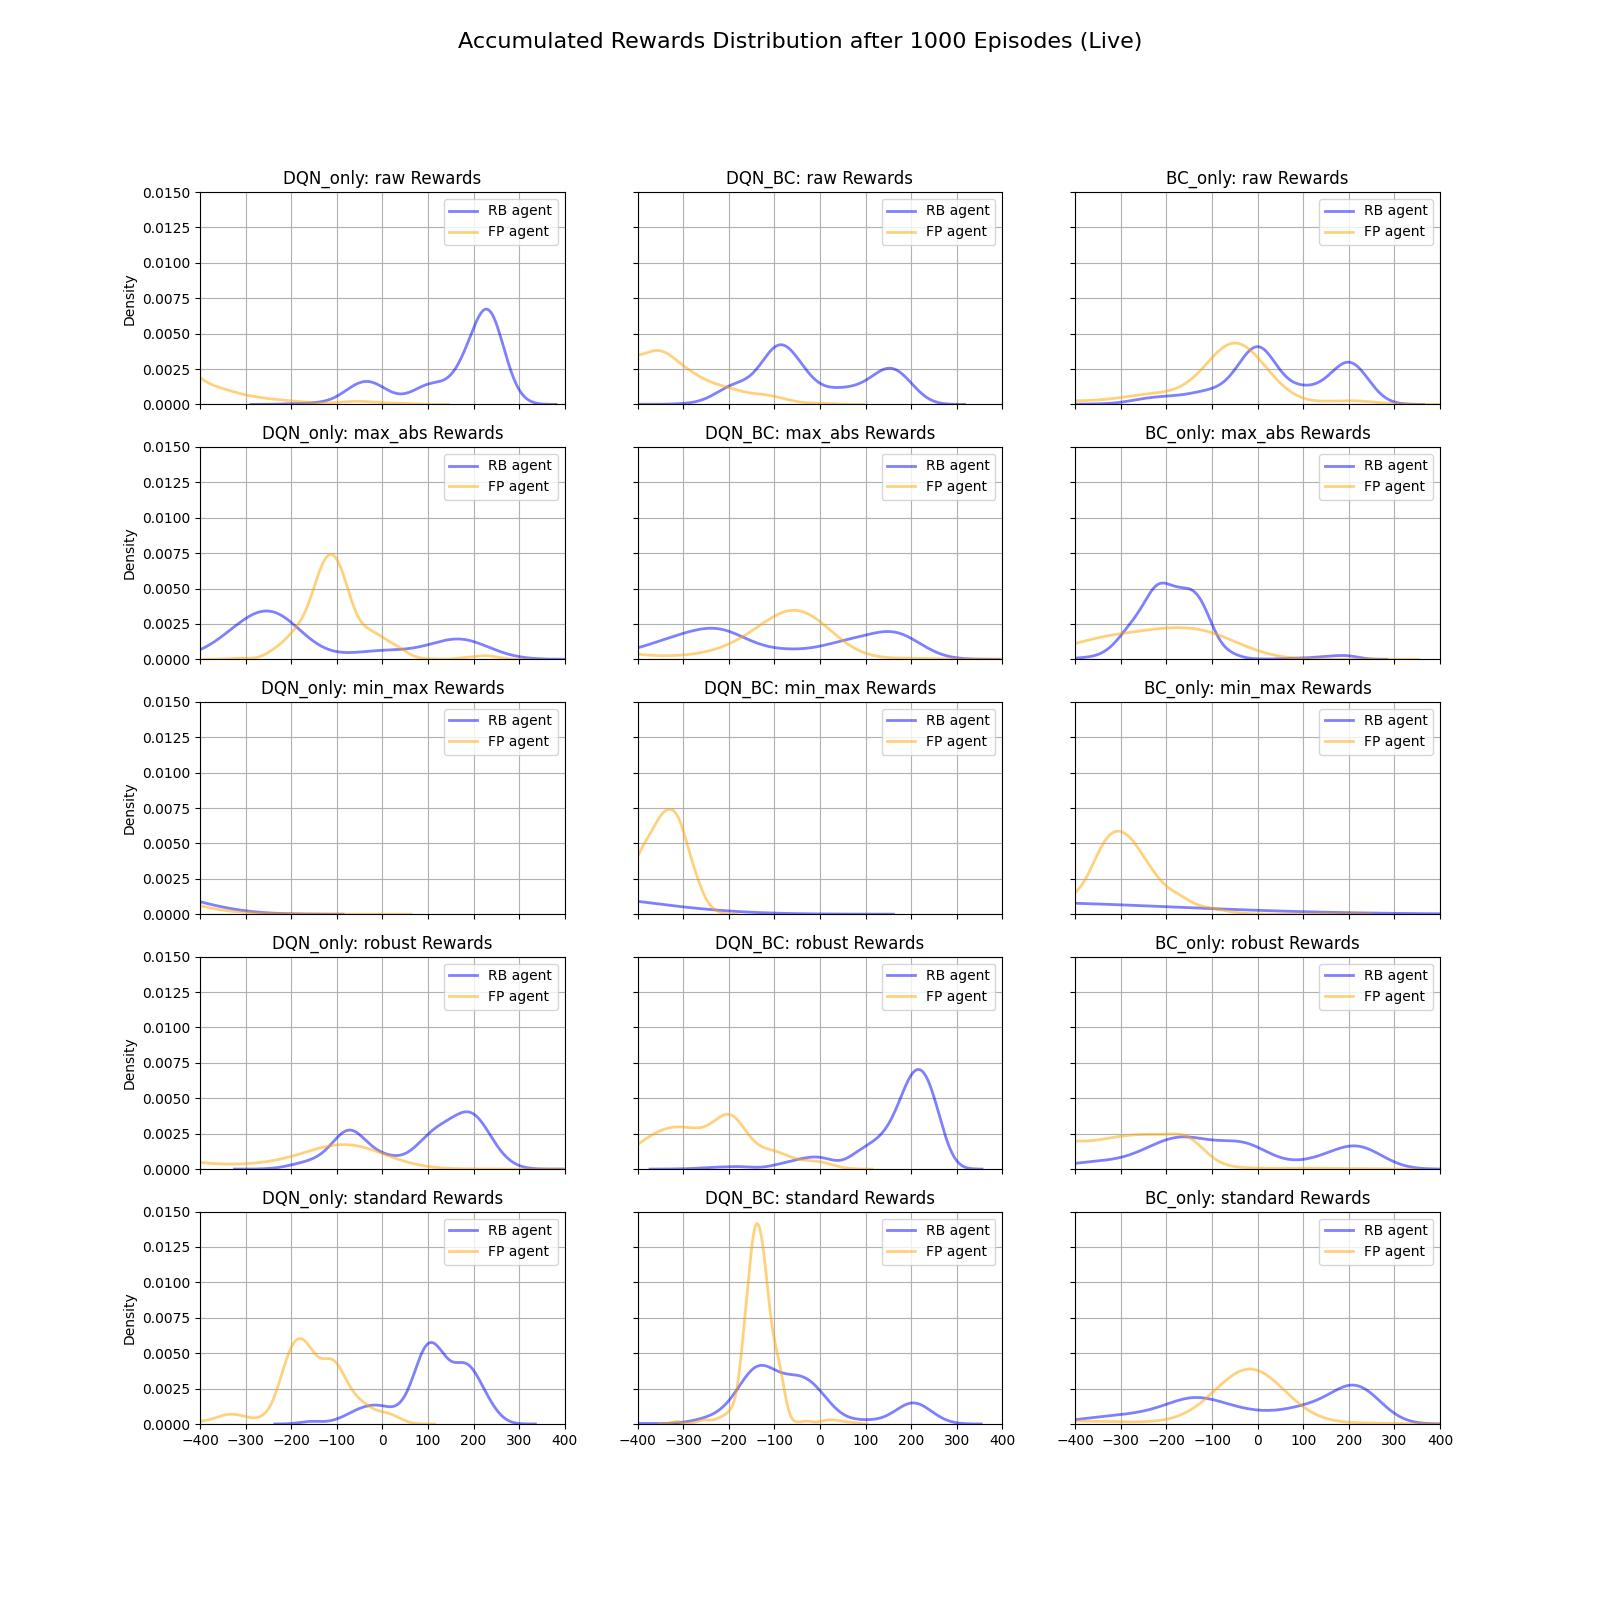
\includegraphics[width=1.15\linewidth, trim=0.75cm 1cm 0.75cm 0cm, clip]{images/DQN_BC_experiments_summary_live_env_1000_ep_eval_rb_fp.jpg}
\caption{
KDEs of accumulated reward distributions for all 30 DQN+BC offline RL agent configurations, evaluated in the live environment over the same 1,000 uniquely seeded episodes. For clarity, reward distributions are plotted within the range $[-400, 400]$.
}
\label{fig:DQN_BC_live_env_evaluation}
\end{figure}

\subsection{Impact of Dataset Composition on Offline DQN+BC (RB vs FP)}
In contrast to the supervised BC models, the dataset training choice had a significantly different impact on the performance of offline DQN+BC agents. Across almost all configurations, agents trained on the RB dataset consistently outperformed those trained on the FP dataset, regardless of the type of regularization applied. This pattern held for all variations (DQN-only, DQN+BC, and BC-only), suggesting that the advantage of RB comes from the dataset itself, not from how the BC regularization is configured, tuned or how well performs.


RB-based agents achieved higher accumulated rewards than FP-based agents across almost all normalization methods, with the only exception being the Min-Max normalization variant. Importantly, this performance advantage was observed even though the supervised BC models trained on RB data were worse at imitation than those trained on FP. This indicates that the effect of the data set is related to the offline RL process and not a consequence of the quality of the BC models` or the regularization configuration.

A likely explanation for this phenomenon comes from the TD-based nature of DQN. TD-learning benefits from the presence of sub-optimal or exploratory state-action pairs, which provide informative gradients for value estimation. Such transitions reduce overestimation and extrapolation error by anchoring value estimates across a wider region of the state–action space. The RB dataset, generated by multiple exploratory or sub-optimal policies, contains a rich set of such transitions. In contrast, the FP dataset is produced by a single near-optimal policy, resulting in a less diverse set of state-action pairs. This lack of sub-optimal examples limits the ability of FP-trained DQN+BC agents to explore value estimates effectively, reducing their overall performance.

These findings are consistent with prior works in offline RL, which highlights that dataset diversity and coverage of the state-action space are critical for stable and reliable value learning \cite{dataset_composition_rl_effects}. In this setting, the RB dataset provides the exploratory breadth necessary for TD-based updates to generalize well, while FP datasets offer insufficient variance to achieve the same level of performance.

The KDE plots of accumulated rewards in the live environment, presented in Figure~\ref{fig:DQN_BC_live_env_evaluation}, clearly show that RB-trained agents perform better. RB-based configurations consistently achieve higher and more concentrated reward peaks compared to FP-based agents, confirming that the composition of the data set is a key factor in offline DQN+BC performance.





\subsection{Effect of State Normalization on Offline DQN+BC Performance}
Unlike the supervised BC models, state normalization had a notable effect on the performance of offline DQN+BC agents. Across the tested configurations, normalization generally improved outcomes for RB-based agents, although some FP-based configurations also saw small gains.

Among the normalization techniques, robust normalization proved to be the most effective in this experimental setup, particularly for DQN+BC agents where $\tau$ was treated as a hyperparameter. Standard normalization also yielded improvements, but slightly less pronounced. In contrast, Max-Abs normalization offered little to no improvements for FP-based agents and could even degrade performance for RB-based agents when compared to raw state inputs. Min-Max normalization failed entirely across all datasets and regularization setups.

The varying success of these normalization methods suggests that certain aspects of the state dimensions (such as the sign of individual features) carry important semantic meaning that can be disrupted or lost by some normalization techniques. These results indicate that even when using FNNs, normalization is not universally beneficial and must be applied with care.









\subsection{Influence of the Extrapolation Error and Initial State Variability}
Visual inspection of the best-performing DQN+BC agent, more precisely the robust RB configuration, showed that it occasionally fails catastrophically at the very start of some episodes. In these cases, the agent presented unstable behaviour, such as spinning uncontrollably immediately after the start of the episode.

These failures can be traced to two factors. Firstly, offline RL agents are prone to extrapolation error when encountering states that are not well represented in the training data \cite{lange2012batch}. Secondly, the Lunar Lander environment introduces small random forces at the start of each episode, as described in Section \ref{sec:the_lunar_lande_environment}, leading to randomized initial states, for example in linear and angular velocities \cite{LunarLanderEnv}.

When the agent is initialized in such out-of-distribution or entirely unseen states, it is unable to generate stable control from the start, which results in almost immediate failure. This behavior highlights the sensitivity of offline-trained agents to distributional mismatch at episode initialization and highlights the challenges of deploying offline RL agents in environments with some level of stochasticity even if such environments are generally deterministic.






\subsection{Impact of Separating Supervised BC Regularization Training from DQN+BC Training}
Training the supervised BC models separately from the DQN+BC pipeline offers several practical advantages that leads directly into improved performance. By decoupling BC training from DQN+BC training, we can use larger batch sizes and epoch-based training for the BC models, while employing smaller mini-batches during DQN+BC training to better suit the nature of supervised classification training and TD-based learning respectively. For this experimental setup, using a batch size of 128 for BC training and 64 for DQN+BC results in a significant increase in performance for both pipelines.

This separation also allows the application of different pruning strategies adapted to the needs of each training phase. In particular, a Median Pruner is used for supervised BC training, while a Percentile Pruner is applied during DQN+BC training. The Percentile Pruner is less aggressive, making it more suitable for the noisy gradients and high-variance reward signals encountered in DQN+BC optimization. In contrast, using a Median Pruner for DQN+BC training leads to excessive pruning, which effectively sets back learning.


By training BC models independently, we avoid the need to compromise between the quality of the generative model and the stability of value-learning, which is a common challenge in traditional end-to-end DQN+BC pipelines. Here, these benefits, including but not limited to batch size and pruning strategy changes, are made with minimal adjustments to the codebase, allowing each component to be optimized under conditions best suited to its characteristics.  

